\section{Learning image synthesizability} 
In this section, we investigate what visual features contribute to
image synthesizability. Below, we first introduce all features we
considered, and then the regression methods we used for the learning.
% We do not assume the category of textures to be handled, and
% use/design general texture features for the learning.

\subsection{Features}
We start from general image features and then to deliberately designed
ones.

\textbf{Wavelet features}. Wavelets have been widely used for texture
analysis, so we analyze its contribution to image
synthesizability. The complex pyramid wavelet transform on $4$ pyramid
levels, with the sp3Filters is used, due to its promising performance
on texture analysis/synthesis~\cite{Portilla:2000:IJCV}.

\textbf{Self-similarity}. Textures are self-similar in local
appearance, thus it is interesting to evaluate the self-similarity
feature~\cite{self:similarity}, which analyzes the statistics of
internal similarities of local patches. We averaged the self-similarity
vectors of all pixels in an image to represent its self-similarity.

\textbf{Complexity}. We follow~\cite{image:interestingness} to measure
the complexity of an image by comparing the its JPEG compressed size
against its uncompressed size. The feature is quite intuitive -- the
mechanism of JPEG compression is similar to human visual system, thus
the lower the compression rate, the more complex is the texture
pattern.

\textbf{Colorfulness}. The complexity of a texture can be also
reflected by its colorfulness -- it is commonly true that the more
colorful the texture (more colors involved in the texture patterns),
the more complex the texture patterns. We measure colorfulness the
same way as proposed by Datta and Wang~\cite{aesthetic:eccv06}, \ie
the Earth Mover distance of the color histogram of the texture image
to a uniform color histogram (represent the most colorful image), thus
the smaller the distance, the more colorful (complex) the texture.

% \textbf{Entropy}.  To capture the complexity of an image, image
% entropy is also measured. Entropy is a statistical measure of
% randomness that can be used to characterize the texture of the input
% image.

% \textbf{structures} cf.~\cite{tsmoothing2012}: texture and main
% structure exhibit completely different properties, makign them
% surprisingly decomposable. We do not assume specific regularity and
% symmetry of the texture patterns: non-uniform and anistropic texture,
% can be handled in a unified framework.

% We do not assume or manually determine the type of textures, as the
% patterns could vary a lot in different examples. 

% Relative Total Variation (RTV) is simple and yet very effective to
% make main structures stand out, thanks to the characteristics of $D$
% and $\phi$.

\textbf{Patch PCA}.  The randomness of a texture is signaled by the
intrinsic dimensionality of local patches from the texture image.
Patches from random textures normally have higher intrinsic
dimensionality than patches from smooth textures. Therefore, we
perform principal component analysis on local patches sampled from the
texture image and use their intrinsic dimensionality as a feature.
Specifically, we sampled patches of $20\times 20$ pixels, centered at
every pixels of the image, and searched for the dimensionality that
keep $85\%$ of the energy. This intrinsic dimensionality normalized by
original dimensionality of the patches, i.c. $400$, is used as the
score of the regularity of the textures. This feature has been used
already for image quality prediction~\cite{blind:quality:cvpr11}.

\textbf{Textureness}. There is no denying that images of objects and
scenes (e.g. cows and kitchens) are more difficulty to synthesize than
image of textures. Therefore, we train a classifier to distinguish
textures from objects and scenes. The UIUC background dataset and
Brodatz texture dataset are used to represent general objects and
textures. SVMs are used as the classifier with intensity statistics of
patches as features~\cite{material:pami:09}. $5 \times 5$ patches are
used with $200$ centres obtained by k-means method. The classification
score is taken as the feature textureness. 

\begin{figure} [!t]
  \centering
   $ \begin{array}{cccc}
\hspace{-1.5mm}
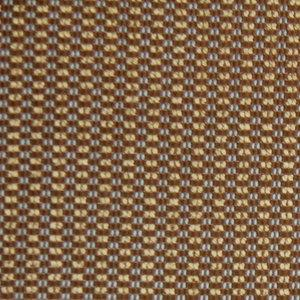
\includegraphics[width=0.33\linewidth]{./figs/repet/1.jpg} & 
\hspace{-3mm}
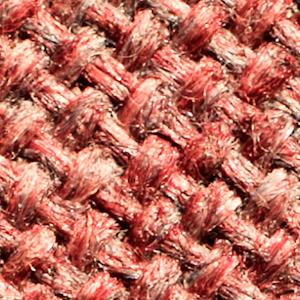
\includegraphics[width=0.33\linewidth]{./figs/repet/273.jpg} & 
\hspace{-3mm}
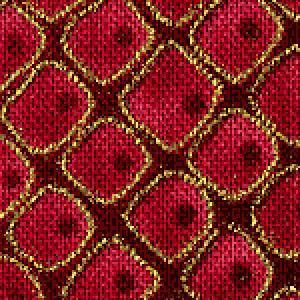
\includegraphics[width=0.33\linewidth]{./figs/repet/352.jpg} \\ 
\scriptsize{\text{repet: 0.99}} & \scriptsize{\text{repet: 0.84}} & \scriptsize{\text{repet: 0.69}}  \\
\hspace{-1.5mm}
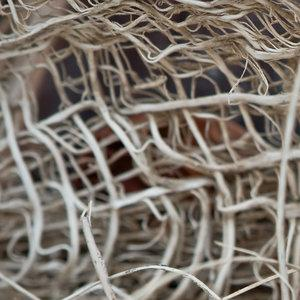
\includegraphics[width=0.33\linewidth]{./figs/repet/439.jpg} & 
\hspace{-3mm}

\includegraphics[width=0.33\linewidth]{./figs/repet/709.jpg} & 
\hspace{-3mm}
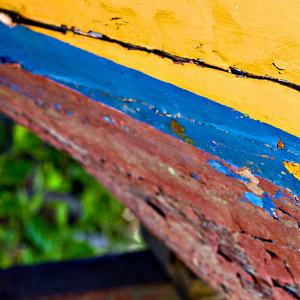
\includegraphics[width=0.33\linewidth]{./figs/repet/832.jpg} \\ 
\scriptsize{\text{repet: 0.52}} & 
\scriptsize{\text{repet: 0.33}} & 
\scriptsize{\text{repet: 0.11}}  \\

\end{array}$
\caption{The repetitiveness of texture examples detected by our
  method. Images are all of $300 \times 300$ pixels.}
  \label{fig:repet}
\end{figure}

\textbf{Edge coverage}.  

\textbf{Attributes} lined or circled~\cite{semantic:texture}? 

\textbf{Repetitiveness}.  Textures are usually referred to as visual
surfaces composed of repeating patterns, that are similar in
appearance and local statistics~\cite{WLKT09}. Although repetitiveness
is a crucial property of textures, it is surprised that there has been
no previous work on estimating it as a general image property. The
closest work is~\cite{autoRectify_12}, where Aiger \etal exploited the
repetition of textures for image rectification. 

Our philosophy is that repetitiveness of an image can be quantified as
the expected (average) amount of information shared by two different
(randomly chosen) regions of the image -- the more the shared
information, the higher the repetitiveness of the image. In
particular, given an image $X \in \mathbb{R}^{H\times W}$, we measure the average shared
information of $T$ trails.  In trial $t$, two image
regions $R_1^t$ and $R_2^t$ are sampled from $X$, and their mutual
information $I_t(R_1^t, R_2^t)$ is measured. The repetitiveness of $X$
is then signaled as
\begin{equation}
  \label{eq:repet}
\text{Rep}(X) = \frac{1}{T}\sum_{t=1}^T I_t(R_1^t, R_2^t).  
\end{equation}
$R_1^t$ and $R_2^t$ are of the same size $H/3 \times W/3$, and their
positions are sampled uniformally, at random from $\{(i,j): i\in\{1,
..., 2H/3\}, j\in \{1, ..., 2W/3\} \}$. Images (regions) are
represented with bag-of-words. The dictionary is learned from $X$ by
k-means with $30$ centres on patches of size $12\times 12$ centered at
every pixel. In order to have an intuitive value, we sort ascendingly
Rep$(X)$ of all $X$'s in our texture dataset and linearly map them to
range $[0, 1]$. The repetitiveness of a new image is calibrated with
the sorting. See Fig.~\ref{fig:repet} for the repetitiveness of some
texture examples detected by the method.

%  \textbf{low-rank texture} 
% Our intuitive distinction between these two kinds
% of data is that textur
% ~\cite{low:rank:texture:ijcv12}. 

\textbf{Regularity}. Inspired by work~\cite{Liu:2004:NTA}, we also
conjecture that the regularity (irregularity) of textures is relevant
to their synthesizability. Although Liu \etal~\cite{Liu:2004:NTA}
proposed a decade ago that textures can be organized by their
regularity (irregularity), there has been no method yet to measure
this computationally. We propose Ensemble Composition (EI) to address
this problem. The idea is that if a texture is regular, it will be
easy to compose its regions using image chunks outside the regions. We
again do this in an ensemble $T$ of trials, and use the reverse
average composition energy to indicate texture regularity. In the $t$
trial, given an image $X$, we denote by $R^t$ the region to composite,
and $Y^t$ the rest of the image. The composition should have two
properties: (1) the composited version should be as similar to $R^t$ as
possible; (2) the chunks from $Y^t$ should be as continous (large) as
possible. It is straightforward to formulate the composition as
a graph labeling problem, with pixel positions of $Y^t$ as labels and
pixel values of $R^t$ as observed data. The formulation is:
\begin{equation}
  \label{eq:regu:energy}
  E(R^t) = \sum_{i\in R^t}D_i(l_i) + \lambda \sum_{\{i,j\} \in \mathcal{N}}V(l_i, l_j)
\end{equation}
where $l_i \in \{1, ..., \#(Y^t)\}$ is the label assigned to pixel $i$
in region $R^t$, and $\mathcal{N}$ is neighborhood set of image
pixels. $D_i(l_i)$ denotes the cost of assigning the $l_i$th pixel of
$Y^t$ to the $i$th pixel position of $R^t$, and is defined as the
Euclidean distance of the RGB values of the $l_i$th pixel of $Y^t$ and
the $i$th pixel in $R^t$. For the smoothing term $V(l_i, l_j)$, we use
the Potts model, i.c. $V(l_i,l_j) = 0$ if $\mathbf{s}(i,
j)=\mathbf{s}(l_i,l_j)$ and $1$ otherwise, where $\mathbf{s}(\cdot,
\cdot)$ is the shift vector between two positions.

By performing $T$ trials, the regularity of texture $X$ is then
defined as:
\begin{equation}
  \label{eq:regularity}
  \text{Reg}(X) = \frac{1}{\frac{1}{T} \sum_{t=1}^{T}E(R^t)}
\end{equation}


optimization using eccv12 paper's technique~\cite{He:completion:eccv12}. 


To avoid the influcence of image cotent to the unary energy (\eg
smooth images aways have smaller energy than ...), we use histogram equalization technique to ...
in order to be dominated by smooth textures, we use histogram
equalization to fill all the range.  Regularity is regular, what we
detected and if it is not no regular.

\begin{figure} [!t]
  \centering
   $ \begin{array}{cccc}
\hspace{-1.5mm}
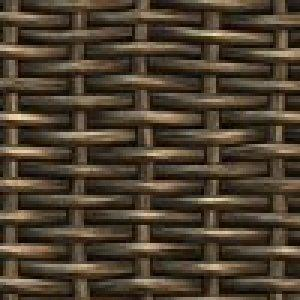
\includegraphics[width=0.33\linewidth]{./figs/regularity/57.jpg} & 
\hspace{-3mm} 
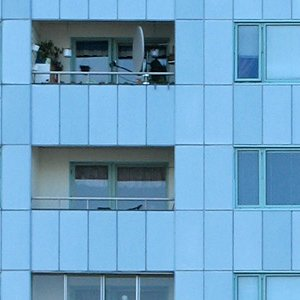
\includegraphics[width=0.33\linewidth]{./figs/regularity/facade.jpg} & 
\hspace{-3mm}

\includegraphics[width=0.33\linewidth]{./figs/regularity/83.jpg} \\ 
\scriptsize{\text{regul: 0.98}} & \scriptsize{\text{regul: 0.87}} & \scriptsize{\text{regul: 0.66}}  \\
\hspace{-1.5mm}
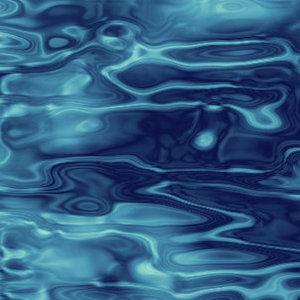
\includegraphics[width=0.33\linewidth]{./figs/regularity/40.jpg} & 
\hspace{-3mm}
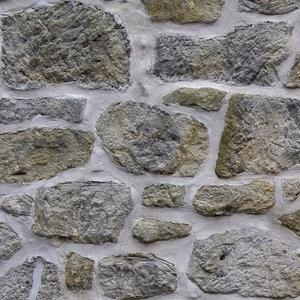
\includegraphics[width=0.33\linewidth]{./figs/regularity/13.jpg} & 
\hspace{-3mm}
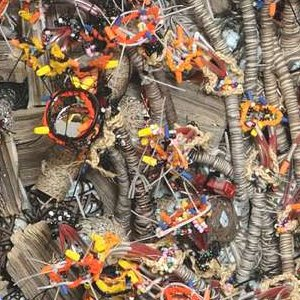
\includegraphics[width=0.33\linewidth]{./figs/regularity/22.jpg} \\ 
\scriptsize{\text{regul: 0.50}} & 
\scriptsize{\text{regul: 0.23}} & 
\scriptsize{\text{regul: 0.08}}  \\

\end{array}$
\caption{The regularity of texture examples captured by ensemble
  inpainting. Images are all of $300 \times 300$ pixels.}
  \label{fig:regularity}
\end{figure}


%\textbf{Shape From Shading}



